\documentclass[aspectratio=169,10pt]{beamer}

% ─── Theme & Colors ────────────────────────────────────────────────────────────
\usetheme{Madrid}
\usecolortheme{default}

\definecolor{darkblue}{HTML}{0D1B2A}
\definecolor{accent}{HTML}{00B4D8}
\definecolor{accentlight}{HTML}{90E0EF}
\definecolor{danger}{HTML}{EF233C}
\definecolor{success}{HTML}{06D6A0}
\definecolor{warn}{HTML}{FFB703}
\definecolor{codebg}{HTML}{1A1A2E}
\definecolor{textlight}{HTML}{CAF0F8}
\definecolor{phasebg0}{HTML}{E0F7FA}
\definecolor{phasebg1}{HTML}{FDECEF}
\definecolor{phasebg2}{HTML}{FFF8E1}
\definecolor{phasebg3}{HTML}{E8F5E9}

\setbeamercolor{palette primary}{bg=darkblue,fg=accent}
\setbeamercolor{palette secondary}{bg=darkblue!90,fg=white}
\setbeamercolor{palette tertiary}{bg=darkblue!80,fg=white}
\setbeamercolor{palette quaternary}{bg=darkblue,fg=white}
\setbeamercolor{structure}{fg=accent}
\setbeamercolor{block title}{bg=accent,fg=darkblue}
\setbeamercolor{block body}{bg=darkblue!8,fg=darkblue}
\setbeamercolor{block title alerted}{bg=danger,fg=white}
\setbeamercolor{block body alerted}{bg=danger!8,fg=black}
\setbeamercolor{block title example}{bg=success!80!black,fg=white}
\setbeamercolor{block body example}{bg=success!8,fg=black}
\setbeamercolor{frametitle}{bg=darkblue,fg=accent}
\setbeamercolor{background canvas}{bg=white}
\setbeamercolor{normal text}{fg=darkblue}
\setbeamercolor{footline}{bg=darkblue,fg=accentlight}

\setbeamertemplate{navigation symbols}{}
\setbeamertemplate{headline}{}

% ─── Footline ──────────────────────────────────────────────────────────────────
\setbeamertemplate{footline}{%
  \leavevmode%
  \begin{beamercolorbox}[wd=\paperwidth,ht=0.1pt]{accent}%
  \end{beamercolorbox}%
  \hbox to \paperwidth{%
    \begin{beamercolorbox}[wd=.3333\paperwidth,ht=3.25ex,dp=1.5ex,leftskip=8mm]{footline}%
      \usebeamerfont{footline}\tiny \textbf{GROUP 19} \;\textbar\; Laksh M. et al.%
    \end{beamercolorbox}%
    \begin{beamercolorbox}[wd=.3333\paperwidth,ht=3.25ex,dp=1.5ex,center]{footline}%
      \usebeamerfont{footline}\tiny INFRASTRUCTURE VULNERABILITY ANALYSIS%
    \end{beamercolorbox}%
    \begin{beamercolorbox}[wd=.3334\paperwidth,ht=3.25ex,dp=1.5ex,rightskip=8mm,right]{footline}%
      \usebeamerfont{footline}\tiny \insertframenumber{} / \inserttotalframenumber%
    \end{beamercolorbox}%
  }%
  \vskip0pt%
}

% ─── Packages ──────────────────────────────────────────────────────────────────
\usepackage{tikz}
\usetikzlibrary{arrows.meta,shapes.geometric,positioning,calc,fit,backgrounds,shadows}
\usepackage{fontenc}
\usepackage{inputenc}
\usepackage{lmodern}
\usepackage{microtype}
\usepackage{xcolor}
\usepackage{listings}
\usepackage{array}
\usepackage{booktabs}

% ─── TikZ Styles ───────────────────────────────────────────────────────────────
\tikzset{
  actor/.style={
    rectangle, rounded corners=5pt,
    draw=accent, line width=1.5pt,
    fill=darkblue, text=white,
    font=\bfseries\small,
    minimum height=12mm, minimum width=32mm,
    align=center, drop shadow={opacity=0.3}
  },
  phaselabel/.style={
    rectangle, rounded corners=3pt,
    font=\scriptsize\bfseries,
    minimum width=16mm, minimum height=6mm,
    inner sep=2pt, align=center
  },
  arr/.style={-{Stealth[length=6pt,width=4pt]}, line width=1.3pt},
  infobox/.style={
    rectangle, rounded corners=4pt,
    line width=1pt, font=\tiny,
    inner sep=5pt, align=left, text width=3.8cm
  },
  mitigate/.style={
    rectangle, rounded corners=4pt,
    draw=success!70!black, line width=1.2pt,
    fill=success!8, font=\scriptsize\bfseries,
    inner sep=5pt, align=left, text=darkblue
  },
}

% ─── Metadata ──────────────────────────────────────────────────────────────────
\title[HTTP/1.1 Request Smuggling]{\textbf{Infrastructure Vulnerability Analysis}\\[2pt]
  \large HTTP/1.1 Request Smuggling \& Mitigation}
\subtitle{Web Cache Poisoning via CL.TE Desynchronization}
\author[Group 19]{%
  \textbf{Group 19}\\[3pt]
  \scriptsize
  Laksh Mendpara \quad Sahilpreet Singh \quad Saher Dev\\
  Aaditya Bansal \quad Anshuman Parida
}
\date{05.07.2025}
\institute[]{Cybersecurity Laboratory}

% ═══════════════════════════════════════════════════════════════════════════════
\begin{document}
% ═══════════════════════════════════════════════════════════════════════════════

% ─── SLIDE 1: TITLE ────────────────────────────────────────────────────────────
{%
\setbeamertemplate{footline}{}%
\begin{frame}[plain]
  \begin{tikzpicture}[remember picture, overlay]
    % Background
    \fill[darkblue] (current page.south west) rectangle (current page.north east);
    % Accent rules
    \fill[accent] (current page.north west) rectangle +(\paperwidth, -4pt);
    \fill[accent] (current page.south west) rectangle +(\paperwidth, 4pt);
    % Decorative background
    \foreach \x in {0,2,...,16} {
      \draw[accent!8, line width=0.4pt] (\x, 0) -- (\x, 9);
    }
    \foreach \y in {0,1.5,...,9} {
      \draw[accent!8, line width=0.4pt] (0, \y) -- (16, \y);
    }
    % Title content
    \node[text=white, font=\bfseries\LARGE, align=center] at (current page.center) {%
      \textcolor{accent}{\rule{8cm}{2pt}}\\[10pt]
      \textcolor{accentlight}{\small INFRASTRUCTURE VULNERABILITY ANALYSIS}\\[12pt]
      {\LARGE HTTP/1.1 Request Smuggling}\\[6pt]
      {\large \& Cache Poisoning Mitigation}\\[10pt]
      \textcolor{accent}{\rule{8cm}{2pt}}
    };
    \node[text=accentlight, font=\scriptsize, align=center]
      at ([yshift=-3.0cm]current page.center)
      {CL.TE Desynchronization Attack on a 3-Tier Stack
       (Nginx $\rightarrow$ Varnish $\rightarrow$ Go Backend)};
    \node[text=white, font=\small, align=center]
      at ([yshift=-4.0cm]current page.center)
      {\textcolor{accent}{\textbf{Group 19}} \;\textbar\;
       Laksh Mendpara \;$\cdot$\; Sahilpreet Singh \;$\cdot$\;
       Saher Dev \;$\cdot$\; Aaditya Bansal \;$\cdot$\; Anshuman Parida};
    \node[text=accentlight!50, font=\tiny]
      at ([yshift=-4.7cm]current page.center) {05.07.2025};
  \end{tikzpicture}
\end{frame}
}

% ─── SLIDE 2: ATTACK FLOW ──────────────────────────────────────────────────────
\begin{frame}{\textbf{CL.TE Attack Flow} --- Desynchronization \& Cache Poisoning}
\vspace{-2mm}

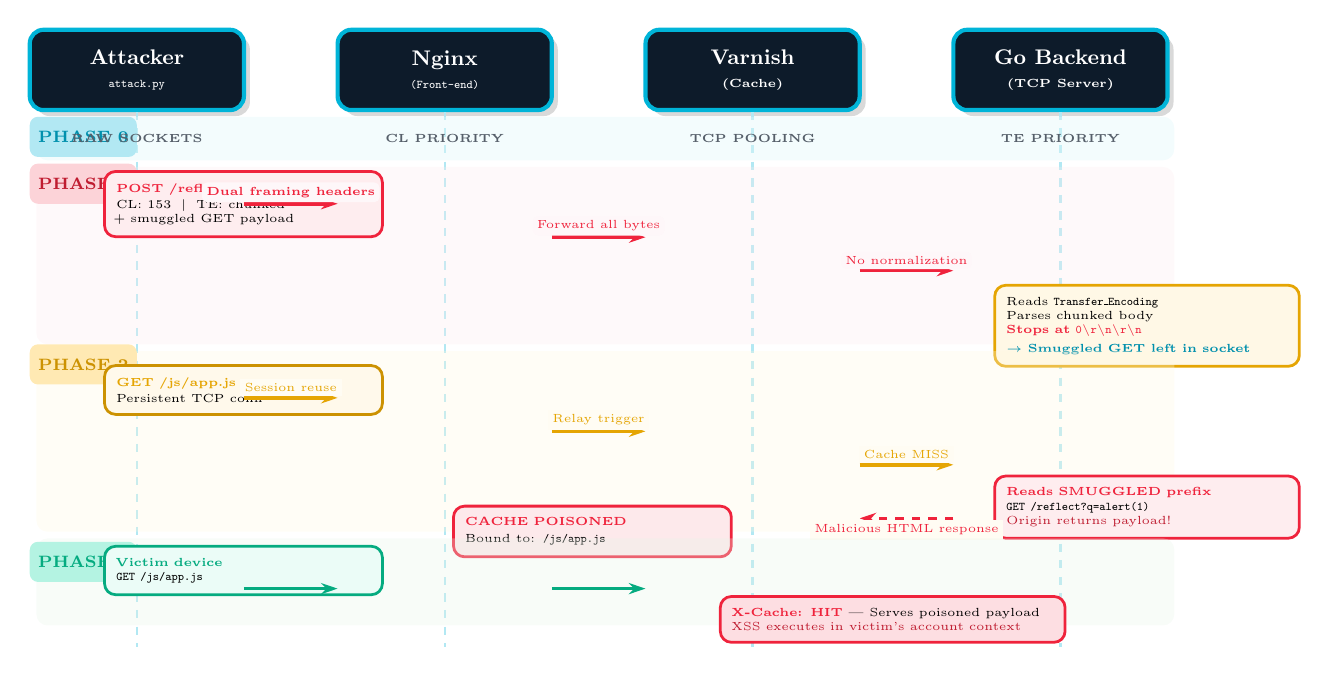
\begin{tikzpicture}[remember picture, scale=0.85, transform shape,
                    every node/.style={transform shape}]

  % ── Column positions (Centering and filling width) ───────────────────────────
  \def\colA{0}        % Attacker
  \def\colB{4.6}      % Nginx
  \def\colC{9.2}      % Varnish
  \def\colD{13.8}     % Go Backend

  % ── Actors ───────────────────────────────────────────────────────────────────
  \node[actor] (A) at (\colA, 0)  {Attacker\\[-1pt]{\tiny\ttfamily attack.py}};
  \node[actor] (N) at (\colB, 0)  {Nginx\\[-1pt]{\tiny\ttfamily (Front-end)}};
  \node[actor] (V) at (\colC, 0)  {Varnish\\[-1pt]{\tiny (Cache)}};
  \node[actor] (B) at (\colD, 0)  {Go Backend\\[-1pt]{\tiny (TCP Server)}};

  % ── Lifelines ────────────────────────────────────────────────────────────────
  \foreach \n in {A,N,V,B} {
    \draw[dashed, accent!30, line width=0.8pt] (\n.south) -- ++(0,-8.0);
  }

  % ════════════════════════════════════════════════════════════════════════════
  % PHASE 0 — Environment
  % ════════════════════════════════════════════════════════════════════════════
  \fill[phasebg0, rounded corners=4pt, opacity=0.4]
    (-1.5,-0.7) rectangle (15.5,-1.35);
  \node[phaselabel, fill=accent!30, text=accent!80!black] at (-0.8,-1.0)
    {PHASE 0};
  \node[font=\tiny\bfseries, text=darkblue!70] at (\colA,-1.02) {RAW SOCKETS};
  \node[font=\tiny\bfseries, text=darkblue!70] at (\colB,-1.02) {CL PRIORITY};
  \node[font=\tiny\bfseries, text=darkblue!70] at (\colC,-1.02) {TCP POOLING};
  \node[font=\tiny\bfseries, text=darkblue!70] at (\colD,-1.02) {TE PRIORITY};

  % ════════════════════════════════════════════════════════════════════════════
  % PHASE 1 — CL.TE Injection
  % ════════════════════════════════════════════════════════════════════════════
  \fill[phasebg1, rounded corners=4pt, opacity=0.3]
    (-1.5,-1.45) rectangle (15.5,-4.1);
  \node[phaselabel, fill=danger!20, text=danger!80!black] at (-0.8,-1.7)
    {PHASE 1};

  % Attacker → Nginx
  \node[infobox, fill=danger!8, draw=danger, anchor=north west]
    (pkt) at (\colA-0.5,-1.5)
    {\textcolor{danger}{\textbf{POST /reflect}}\\[1pt]
     CL: 153 \;\textbar\; TE: chunked\\
     + smuggled GET payload};

  \draw[arr, danger] (\colA+1.6,-2.0) -- node[above, font=\tiny, fill=phasebg1!40,
    inner sep=2pt, rounded corners=2pt]{\textbf{Dual framing headers}} (\colB-1.6,-2.0);

  % Nginx → Varnish
  \draw[arr, danger] (\colB+1.6,-2.5) -- node[above, font=\tiny, fill=phasebg1!40,
    inner sep=2pt, rounded corners=2pt]{Forward all bytes} (\colC-1.6,-2.5);

  % Varnish → Backend
  \draw[arr, danger] (\colC+1.6,-3.0) -- node[above, font=\tiny, fill=phasebg1!40,
    inner sep=2pt, rounded corners=2pt]{No normalization} (\colD-1.6,-3.0);

  % Backend action
  \node[infobox, fill=warn!10, draw=warn!90!black, anchor=north west,
        text width=4.2cm]
    (bact) at (\colD-1.0,-3.2)
    {Reads \texttt{Transfer\_Encoding}\\
     Parses chunked body\\
     \textcolor{danger}{\bfseries Stops at \texttt{0\textbackslash r\textbackslash n\textbackslash r\textbackslash n}}\\[2pt]
     \textcolor{accent!80!black}{\bfseries $\rightarrow$ Smuggled GET left in socket}};

  % ════════════════════════════════════════════════════════════════════════════
  % PHASE 2 — Trigger + Cache Poisoning
  % ════════════════════════════════════════════════════════════════════════════
  \fill[phasebg2, rounded corners=4pt, opacity=0.3]
    (-1.5,-4.2) rectangle (15.5,-6.9);
  \node[phaselabel, fill=warn!30, text=warn!80!black] at (-0.8,-4.4)
    {PHASE 2};

  % Attacker trigger
  \node[infobox, fill=warn!8, draw=warn!80!black, anchor=north west]
    at (\colA-0.5,-4.4)
    {\textcolor{warn!90!black}{\textbf{GET /js/app.js}}\\[1pt]
     Persistent TCP conn};

  \draw[arr, warn!90!black] (\colA+1.6,-4.9) --
    node[above, font=\tiny, fill=phasebg2!40, inner sep=2pt]{Session reuse}
    (\colB-1.6,-4.9);

  \draw[arr, warn!90!black] (\colB+1.6,-5.4) --
    node[above, font=\tiny, fill=phasebg2!40, inner sep=2pt]{Relay trigger}
    (\colC-1.6,-5.4);

  \draw[arr, warn!90!black] (\colC+1.6,-5.9) --
    node[above, font=\tiny, fill=phasebg2!40, inner sep=2pt]{Cache MISS}
    (\colD-1.6,-5.9);

  % Backend reads smuggled prefix
  \node[infobox, fill=danger!8, draw=danger, anchor=north west,
        text width=4.2cm]
    at (\colD-1.0,-6.05)
    {\textcolor{danger}{\bfseries Reads SMUGGLED prefix}\\
     \texttt{GET /reflect?q=alert(1)}\\
     \textcolor{danger!80!black}{Origin returns payload!}};

  % Return arrow — poisoned response
  \draw[arr, danger, dashed] (\colD-1.6,-6.7) --
    node[below, font=\tiny, fill=phasebg2!40, inner sep=2pt]
    {\textcolor{danger}{Malicious HTML response}}
    (\colC+1.6,-6.7);

  % Varnish caches
  \node[infobox, fill=danger!10, draw=danger, anchor=north east]
    at (\colC-0.3,-6.5)
    {\textcolor{danger}{\bfseries CACHE POISONED}\\[1pt]
     Bound to: \texttt{/js/app.js}};

  % ════════════════════════════════════════════════════════════════════════════
  % PHASE 3 — Victim
  % ════════════════════════════════════════════════════════════════════════════
  \fill[phasebg3, rounded corners=4pt, opacity=0.3]
    (-1.5,-7.0) rectangle (15.5,-8.3);
  \node[phaselabel, fill=success!30, text=success!80!black] at (-0.8,-7.35)
    {PHASE 3};

  \node[infobox, fill=success!8, draw=success!80!black, anchor=north west]
    at (\colA-0.5,-7.1)
    {\textcolor{success!80!black}{\textbf{Victim device}}\\
     \texttt{GET /js/app.js}};

  \draw[arr, success!80!black] (\colA+1.6,-7.75) -- (\colB-1.6,-7.75);
  \draw[arr, success!80!black] (\colB+1.6,-7.75) -- (\colC-1.6,-7.75);

  \node[infobox, fill=danger!15, draw=danger, anchor=north west,
        text width=4.8cm] at (\colC-0.5,-7.85)
    {\textcolor{danger}{\bfseries X-Cache: HIT}
     --- Serves poisoned payload\\
     \textcolor{danger!80!black}{XSS executes in victim's account context}};

\end{tikzpicture}

\end{frame}

% ─── SLIDE 3: MITIGATION ────────────────────────────────────────────────────────
\begin{frame}{\textbf{Mitigation \& Remediation} --- Closing All Vectors}
\vspace{-1mm}

\begin{columns}[T,totalwidth=\textwidth]

% ── Left: Mitigation flow ─────────────────────────────────────────────────────
\begin{column}{0.46\textwidth}
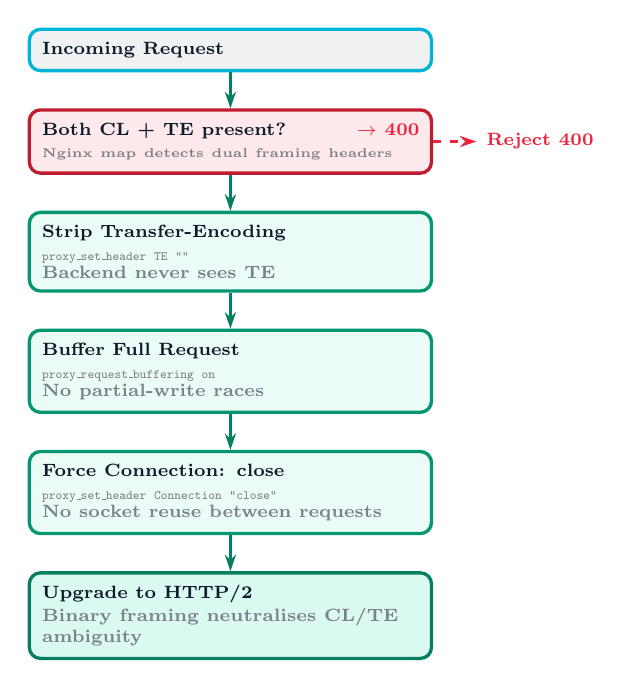
\begin{tikzpicture}[node distance=5mm, scale=0.92, transform shape]

  \node[mitigate, fill=darkblue!6, draw=accent, text width=5.2cm]
    (req) {\textbf{Incoming Request}};

  \node[mitigate, fill=danger!10, draw=danger!80!black, text width=5.2cm,
        below=of req]
    (check) {\textbf{Both CL + TE present?} \hfill
      \textcolor{danger}{\bfseries $\rightarrow$ 400}\\[1pt]
      \textcolor{gray}{\tiny Nginx map detects dual framing headers}};

  \node[mitigate, text width=5.2cm, below=of check]
    (strip) {\textbf{Strip Transfer-Encoding}\\[1pt]
      \textcolor{gray}{\tiny\texttt{proxy\_set\_header TE ""}}\\[-1pt]
      \textcolor{darkblue!55}{\scriptsize Backend never sees TE}};

  \node[mitigate, text width=5.2cm, below=of strip]
    (buf) {\textbf{Buffer Full Request}\\[1pt]
      \textcolor{gray}{\tiny\texttt{proxy\_request\_buffering on}}\\[-1pt]
      \textcolor{darkblue!55}{\scriptsize No partial-write races}};

  \node[mitigate, text width=5.2cm, below=of buf]
    (conn) {\textbf{Force Connection: close}\\[1pt]
      \textcolor{gray}{\tiny\texttt{proxy\_set\_header Connection "close"}}\\[-1pt]
      \textcolor{darkblue!55}{\scriptsize No socket reuse between requests}};

  \node[mitigate, fill=success!15, draw=success!60!black, text width=5.2cm,
        below=of conn]
    (h2) {\textbf{Upgrade to HTTP/2}\\[1pt]
      \textcolor{darkblue!55}{\scriptsize Binary framing neutralises CL/TE ambiguity}};

  % Arrows
  \draw[arr, success!60!black] (req.south) -- (check.north);
  \draw[arr, danger, dashed]
    (check.east) -- ++(0.6,0)
    node[right, font=\scriptsize\bfseries, text=danger]{Reject 400};
  \draw[arr, success!60!black] (check.south) -- (strip.north);
  \draw[arr, success!60!black] (strip.south) -- (buf.north);
  \draw[arr, success!60!black] (buf.south) -- (conn.north);
  \draw[arr, success!60!black] (conn.south) -- (h2.north);

\end{tikzpicture}
\end{column}

% ── Right: Summary + Before/After ─────────────────────────────────────────────
\begin{column}{0.52\textwidth}

\begin{block}{\small Mitigation per Layer}
\vspace{1mm}
{\small
\begin{tabular}{@{}>{\bfseries}p{1.4cm} p{5cm}@{}}
\toprule
Layer & Action \\
\midrule
Nginx &
  \texttt{underscores\_in\_headers on}; map detects dual CL+TE
  $\rightarrow$ 400; strips TE; buffers; forces close \\[3pt]
Varnish &
  Rejects dual-length; \texttt{unset bereq.http.TE};
  \texttt{Connection:close}; no 5xx caching \\[3pt]
Backend &
  Drains CL body when TE absent; prevents socket corruption \\
\bottomrule
\end{tabular}
}
\end{block}

\vspace{1.5mm}

\begin{alertblock}{\small Without mitigation}
\vspace{1mm}
{\ttfamily\tiny
\colorbox{codebg}{\parbox{\dimexpr\linewidth-2\fboxsep-2pt}{%
  \color{accentlight}%
  HTTP/1.1 200 OK \quad X-Cache: HIT\\
  Content-Type: text/html\\[2pt]
  \color{danger}%
  \textless html\textgreater\textless body\textgreater%
  \textless script\textgreater alert('Poisoned!')%
  \textless/script\textgreater\textless/body\textgreater\textless/html\textgreater
}}}
\vspace{1mm}
\end{alertblock}

\vspace{0.5mm}

\begin{exampleblock}{\small With mitigation}
\vspace{1mm}
{\ttfamily\tiny
\colorbox{codebg}{\parbox{\dimexpr\linewidth-2\fboxsep-2pt}{%
  \color{accentlight}%
  HTTP/1.1 400 Bad Request\\
  Content-Type: text/plain\\[2pt]
  \color{success}%
  Ambiguous request rejected -- dual length headers
}}}
\vspace{1mm}
\end{exampleblock}

\vspace{1mm}
\begin{center}
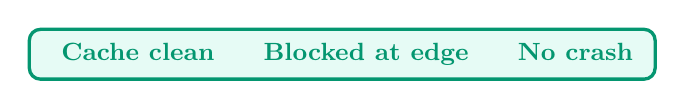
\begin{tikzpicture}
  \node[draw=success!70!black, fill=success!10, rounded corners=4pt,
        line width=1.2pt, font=\small\bfseries, text=success!70!black,
        inner xsep=8pt, inner ysep=5pt]{%
    $\checkmark$ Cache clean \quad
    $\checkmark$ Blocked at edge \quad
    $\checkmark$ No crash};
\end{tikzpicture}
\end{center}

\end{column}
\end{columns}

\end{frame}

\end{document}
